% =====================================================================================================
\section{Background and Threat Model}\label{sec:background}
\textit{Baseline JPEG.} Pixels are converted to YCbCr 4:2:0, so a 16$\times$16 macroblock (MCU) yields six 8$\times$8 blocks, or 1.5 samples per pixel. Each block is transformed by an integer DCT and quantized; the 64 coefficients are read in zig-zag order. The DC coefficient is coded as the difference to the previous block of its component, and each non-zero AC coefficient as a Huffman code for the pair (run of zeros, size category $s$) followed by an $s$-bit appended field~\cite{t81,wallace1992}. For $v \ne 0$,
\begin{equation}
s(v) = \lfloor \log_2 |v| \rfloor + 1, \qquad
\amp(v) = \begin{cases} v, & v > 0,\\ v + 2^s - 1, & v < 0. \end{cases}
\label{eq:amp}
\end{equation}
Two properties follow, and the design rests on both: the field can be changed without changing the Huffman code or the stream length as long as $s$ is kept, and the run lengths and size categories, i.e.\ where the non-zero coefficients are, stay visible to anyone. A restart marker ends a restart segment: the bits are padded to a byte, the DC predictors reset, and the next segment decodes without the previous one~\cite{t81}.

\textit{Ascon-AEAD128.} Ascon~\cite{ascon,sp800232} applies a 320-bit permutation (constant addition, a 5-bit S-box on 64 bit slices, a linear layer of rotations and XORs) to five 64-bit words; Ascon-AEAD128 initializes with 12 rounds from a 128-bit key and nonce, absorbs 128-bit blocks with 8 rounds each and ends with a 128-bit tag. One core serves as a \emph{keystream generator} (the ciphertext of an all-zero message) and as a \emph{MAC} (the tag of an empty message over associated data).

\textit{Threat model.} The attacker sits on the network path: it observes all traffic and may modify, drop, delay, replay, reorder or inject video and feedback datagrams; it knows the design, may know some frames in clear and choose what the camera films, and may train networks on any amount of public video, but holds no key. Physical and side-channel attacks are out of scope. The goals are content confidentiality (no recognisable shape of the scene), integrity and authenticity of every frame with its metadata, freshness, an availability signal (silence counts as an attack), and forward secrecy across key epochs. The last four are enforced cryptographically; confidentiality is a property of the protection level, which we measure.

% =====================================================================================================
\section{Cryptographic Design}\label{sec:design}
\begin{figure*}[t]
\centering
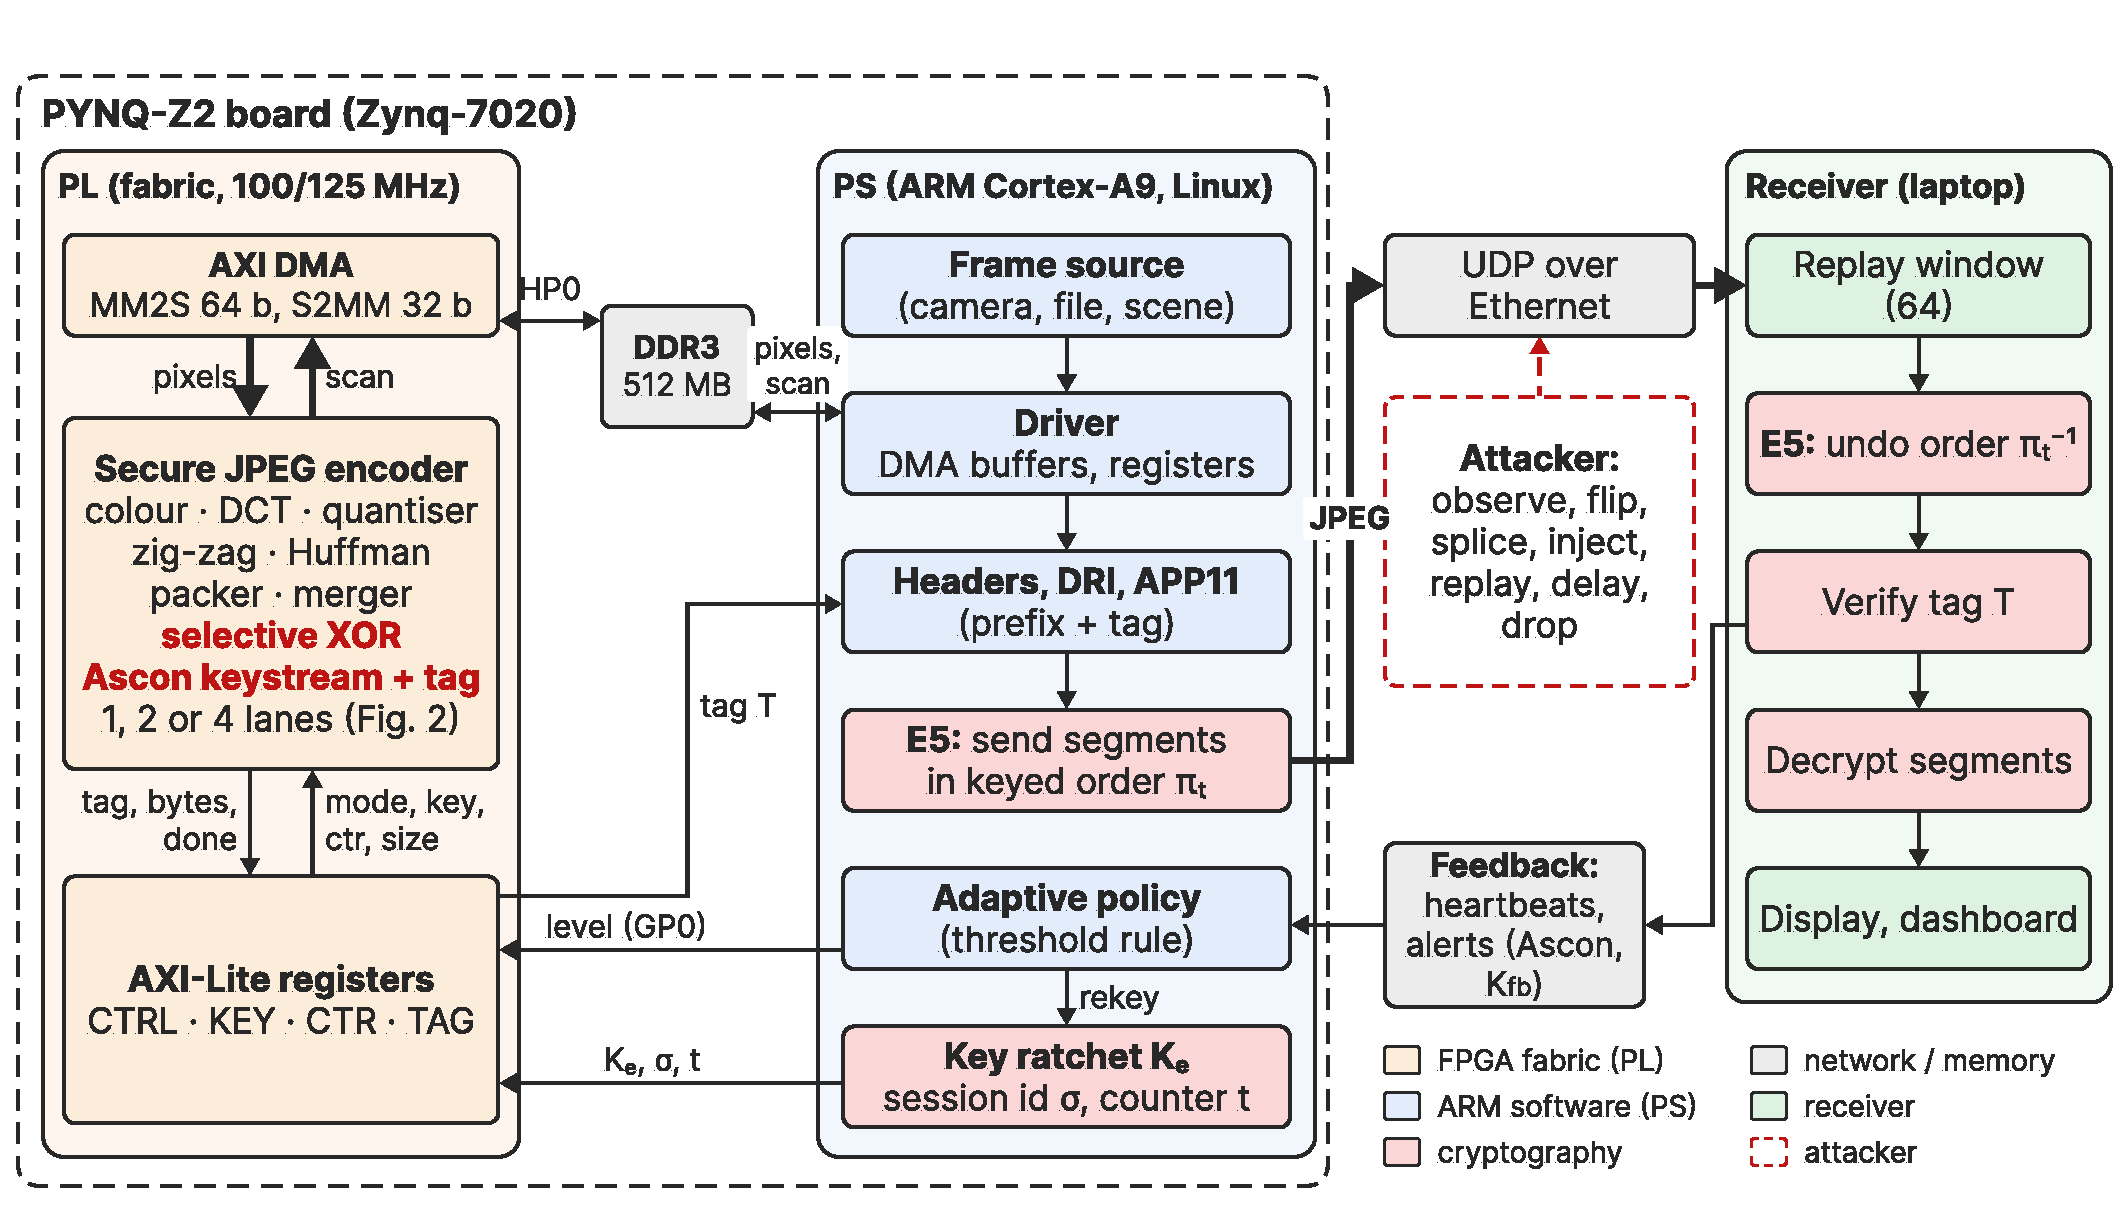
\includegraphics[width=\textwidth]{figures/fig_system.pdf}
\caption{System architecture. The programmable logic (PL) encodes, encrypts and tags every frame; the ARM core (PS) moves pixels and scan through DDR with an AXI DMA, adds the JPEG headers and the tag, sends E5 segments in the keyed order, and runs the key ratchet and the adaptive policy. The receiver undoes the order, verifies the tag, decrypts, and reports back over an authenticated feedback channel. Red: cryptography; dashed: attacker.}
\label{fig:system}
\end{figure*}
Fig.~\ref{fig:system} shows the system. The ARM core places a frame in DDR, writes the per-frame registers and starts the DMA; the fabric codes the pixels into a JPEG scan in which the selected fields are encrypted, computes the frame tag over the metadata and the scan, and writes the scan back. The ARM core wraps it in standard headers and an application segment (APP11) with the tag, reorders the segments under E5, and sends the frame over UDP. All per-byte cryptographic work happens in the fabric.

\subsection{Selective encryption inside the entropy coder}\label{sec:selenc}
\begin{table}[t]
\caption{Protection levels: encrypted fields of every non-zero coefficient (sign: the whole field is inverted; amplitude: its $s{-}1$ low bits) and block positions. Every level carries the tag.}
\label{tab:levels}
\centering\small\setlength{\tabcolsep}{4pt}
\begin{tabular}{lccccc}
\toprule
Level & AC sign & DC sign & AC ampl. & DC ampl. & Positions \\
\midrule
E0 & & & & & \\
E1 & \checkmark & & & & \\
E2 & \checkmark & \checkmark & & & \\
E3 & \checkmark & \checkmark & \checkmark & & \\
E4 & \checkmark & \checkmark & \checkmark & \checkmark & \\
E5 & \checkmark & \checkmark & \checkmark & \checkmark & keyed per frame \\
\bottomrule
\end{tabular}
\end{table}
Table~\ref{tab:levels} lists the six levels; E2 is the default minimum. For a selected symbol with size $s$ and keystream bits $z_0 z_1 \ldots$, the encryption stage computes
\begin{equation}
\amp' = \amp \xor \gamma z_0 (2^s - 1) \xor \alpha \textstyle\sum_{k=1}^{s-1} z_k\, 2^{k-1},
\label{eq:selenc}
\end{equation}
where $\gamma, \alpha \in \{0, 1\}$ say whether the level selects the sign and the amplitude of this coefficient. It consumes $n(s) = \gamma + \alpha (s - 1) \le 11$ keystream bits; decryption is the same XOR.

\begin{lemma}[Format preservation]\label{lem:format}
For every $v \ne 0$ and every keystream, \eqref{eq:selenc} maps $\amp(v)$ to $\amp(v')$ for some $v'$ with $s(v') = s(v)$. Hence the Huffman symbol, the code length and the length of the scan are unchanged, and the encrypted scan is a valid baseline JPEG scan.
\end{lemma}
\begin{IEEEproof}
Let $m = 2^s - 1$. For $v > 0$, $\amp(v) = v$ and $\amp(v) \xor m = m - v = \amp(-v)$ by~\eqref{eq:amp}, and symmetrically for $v < 0$; the sign term is an exact negation. The amplitude term changes only bits $0 \ldots s-2$; bit $s-1$ of $\amp(v)$ is 1 exactly when $v > 0$, and any value of the low bits gives a magnitude in $[2^{s-1}, 2^s - 1]$, i.e.\ size $s$, with the same sign. Neither term touches the run or the Huffman code.
\end{IEEEproof}
The lemma also states what cannot be hidden: the run lengths and size categories stay public at every level E0--E4.

\subsection{Keys, nonces and their uniqueness}\label{sec:nonce}
The master key $K_{\mathrm{m}}$ is the session key that the ARM cores of camera and viewer agree on with a hybrid ML-KEM-768~\cite{fips203} + X25519 exchange authenticated by a pre-shared key. All keys derive from it with one primitive, the Ascon tag used as a pseudorandom function: $\KDF(K, \ell, c) = \MAC_K(N(0, c, 1), \ell)$. The feedback key is $\Kfb = \KDF(K_{\mathrm{m}}, \text{feedback}, 0)$, and the video key follows a one-way ratchet, $K_0 = \KDF(K_{\mathrm{m}}, \text{video}, 0)$, $K_{e+1} = \KDF(K_e, \text{ratchet}, e{+}1)$; each end erases $K_e$ once it has moved on, so a captured key does not decrypt earlier epochs. The 128-bit nonce is
\begin{equation}
N(\sigma, t, b) = \sigma \cat t \cat b, \qquad \sigma = \beta \cat e,
\label{eq:nonce}
\end{equation}
with $\beta$ a 48-bit random base drawn at every boot ($\beta \ne 0$), $e$ the 16-bit epoch, $t$ the 63-bit frame counter and $b$ a purpose bit (0: keystream, 1: tag).

\begin{proposition}[Nonce uniqueness]\label{prop:nonce}
Within one session, no key is used twice with the same nonce, provided the sender never writes the same frame counter twice in an epoch.
\end{proposition}
\begin{IEEEproof}
Under $K_e$ the nonces are $N(\sigma, t, 0)$ for the segment key, $N(\sigma, t, 1)$ for the tag, $N(0, 0, 0)$ for the permutation key and $N(0, c, 1)$ for derivations; $\sigma \ne 0$, $b$ separates the first two, and $t$ is fresh per frame. Under a segment key, a pseudorandom function of $(K_e, \sigma, t)$, the nonces $N(h, t, 0)$ differ in the segment index $h$. A rekey changes both $K_e$ and $\sigma$.
\end{IEEEproof}
With the key exchange every session has a fresh $K_{\mathrm{m}}$. Used directly with the pre-shared key, two boots collide only if they draw the same $\beta$: for $B$ boots this has probability at most $\binom{B}{2} 2^{-48} \approx \BootCollide$ for $B = \BootCount$.

\subsection{Segment keystreams and the frame tag}\label{sec:tag}
Every frame is coded as restart segments (one per MCU row, or one per MCU in E5), each with its own keystream under a per-frame segment key:
\begin{align}
\Kseg &= \MAC_{K_e}\bigl(N(\sigma, t, 0), \text{``lanes''}\bigr), \label{eq:kseg}\\
Z_h &= \Enc_{\Kseg}\bigl(N(h, t, 0), 0^{\ell}\bigr). \label{eq:zs}
\end{align}
Seeking to a segment costs one initialization, which is what lets lanes encrypt independently. The tag authenticates a 26-byte prefix and every byte of the scan, restart markers included:
\begin{equation}
T_t = \MAC_{K_e}\bigl(N(\sigma, t, 1),\ P_t \cat \text{scan}_t\bigr),
\label{eq:tag}
\end{equation}
with $P_t$ = (magic, version, level, $\sigma$, $t$, $W$, $H$). Binding the level matters: an earlier version authenticated only the scan, and a frame could be downgraded from E2 to E1 undetected. The receiver accepts a frame only if~\eqref{eq:tag} verifies and the counter passes a 64-entry replay window as in SRTP~\cite{rfc3711}; a forgery succeeds with probability $2^{-128}$ per attempt.

\subsection{E5: a keyed permutation of macroblocks in hardware form}\label{sec:e5}
\begin{figure}[t]
\centering
\resizebox{\columnwidth}{!}{% E5 in hardware form (docs/INTERFACES.md §8.6): fabric codes MCU segments in raster order and tags them,
% (black bars: restart markers, none after the last segment) the ARM sends them in the keyed order pi_t, the receiver restores raster order before the tag check.
\begin{tikzpicture}[x=1cm, y=1cm,
  seg/.style={draw=inkc, minimum width=5.2mm, minimum height=5.2mm, inner sep=0pt, font=\tiny},
  rst/.style={fill=inkc, minimum width=1.0mm, minimum height=5.2mm, inner sep=0pt},
  st/.style={font=\tiny, align=left, anchor=west}]
\def\segrow#1#2#3{% #1 y, #2 list of labels, #3 fill
  \foreach \l [count=\i from 0] in {#2} {
    \node[seg, fill=#3] at (\i*0.68, #1) {$\l$};
    \ifnum\i<5 \node[rst] at (\i*0.68+0.34, #1) {};\fi
  }}
\segrow{0}{s_0,s_1,s_2,s_3,s_4,s_5}{plfill}
\node[st] at (4.15,0.0) {fabric: one restart segment per MCU, raster order;\\keystream $(K_{\mathrm{seg}}, N_{s,t})$ per segment; $T$ over this order};
\segrow{-1.15}{s_3,s_0,s_5,s_1,s_4,s_2}{cryfill}
\node[st] at (4.15,-1.15) {ARM: send segment $\pi_t(p)$ at position $p$,\\RST renumbered; header and $T$ unchanged};
\segrow{-2.3}{s_0,s_1,s_2,s_3,s_4,s_5}{rxfill}
\node[st] at (4.15,-2.3) {receiver: $\pi_t^{-1}$, then verify $T$,\\then decrypt each segment};
\draw[arr] (-0.45,-0.35) -- node[lbl, left, align=right]{Fisher--Yates\\$\pi_t$} (-0.45,-0.8);
\draw[arr] (-0.45,-1.5) -- node[lbl, left]{$\pi_t^{-1}$} (-0.45,-1.95);
\foreach \a/\b in {0/1,1/3,2/5,3/0,4/4,5/2} {
  \draw[inkc!45, line width=0.3pt] (\a*0.68,-0.27) -- (\b*0.68,-0.88);
}
\end{tikzpicture}
}
\caption{E5 in hardware form. The fabric codes one restart segment per MCU in raster order, each with its own keystream, and tags them in that order; the ARM sends segment $\pi_t(p)$ at wire position $p$; the receiver restores raster order before checking the tag.}
\label{fig:e5}
\end{figure}
Lemma~\ref{lem:format} shows that field encryption cannot hide where the non-zero coefficients are; their count per block alone rebuilds the contours~\cite{hirose2024}. E5 therefore also hides where each macroblock belongs. Permuting macroblocks before entropy coding would need a frame buffer; restart segments allow a cheaper split (Fig.~\ref{fig:e5}). The fabric codes every MCU $h$ as its own segment, encrypted like E4 with $Z_h$, and authenticates the segments in raster order. The ARM splits the scan at the markers and sends segment $\pi_t(p)$ at position $p$, renumbering the markers. The receiver restores raster order with $\pi_t^{-1}$, verifies $T_t$ and only then decrypts. The permutation comes from its own key $K_\pi = \MAC_{K_e}(N(0,0,0), \text{``E5 MCU shuffle''})$ through a Fisher--Yates shuffle on the keystream of $(K_\pi, N(\sigma, t, 0))$, with rejection sampling for uniform indices.

\begin{proposition}[Uniform per-frame permutation]\label{prop:perm}
If the keystream bits are uniform and independent, the shuffle returns each of the $M!$ permutations with probability $1/M!$.
\end{proposition}
\begin{IEEEproof}
At step $i$ a $b_i$-bit draw, $b_i = \lfloor \log_2 i \rfloor + 1$, conditioned on $j \le i$ is uniform on $\{0, \ldots, i\}$; Fisher--Yates with uniform choices produces every permutation exactly once among $\prod_{i=1}^{M-1}(i+1) = M!$ equally likely choice sequences.
\end{IEEEproof}
At 320$\times$240 ($M = \McuQVGA$) the permutation carries $\log_2 M! = \PermBitsQVGA$ bits and costs on average \FyBitsQVGA{} keystream bits. It changes with every frame because $t$ enters the nonce, so the order of one frame says nothing about the next. Because the tag covers the raster-order scan and the receiver derives $\pi_t^{-1}$ from the authenticated $(\sigma, t)$, moving, swapping, dropping or duplicating a segment fails the tag. Each segment adds a two-byte marker, padding and restarted DC prediction, i.e.\ about $M(2 + \tfrac12)$ bytes plus longer DC differences per frame.

\subsection{Authenticated feedback and the adaptive policy}\label{sec:feedback}
The receiver returns an encrypted heartbeat every 0.5\,s and rate-limited alerts (tag failures, replays, malformed or stale frames, loss statistics) under $\Kfb$, with their own counter and replay window. If no valid heartbeat arrives for 3\,s, the sender assumes that the feedback path is attacked: it switches to the highest level and rekeys (dead-man rule). In one-second windows the sender collects the evidence and a threshold policy raises the highest level on any tag failure, replay, feedback attack or flood and holds it for 8\,s; loss counts as jamming only when it is near total, because more encryption cannot help against a degraded network. A contextual bandit~\cite{sutton2018} is the alternative policy: it encrypts fewer bits but reacts later.
